\documentclass[aspectratio=169]{../latex_main/tntbeamer}  % you can pass all options of the beamer class, e.g., 'handout' or 'aspectratio=43'
\usepackage{dsfont}
\usepackage{bm}
\usepackage[english]{babel}
\usepackage[T1]{fontenc}
%\usepackage[utf8]{inputenc}
\usepackage{graphicx}
\graphicspath{ {./figures/} }
\usepackage{algorithm}
\usepackage[ruled,vlined,algo2e,linesnumbered]{algorithm2e}
\usepackage{hyperref}
\usepackage{booktabs}
\usepackage{mathtools}

\usepackage{amsmath,amssymb}

\DeclareMathOperator*{\argmax}{arg\,max}
\DeclareMathOperator*{\argmin}{arg\,min}

\usepackage{pgfplots}
\pgfplotsset{compat=1.16}
\usepackage{tikz}
\usetikzlibrary{trees} 
\usetikzlibrary{shapes.geometric}
\usetikzlibrary{positioning,shapes,shadows,arrows,calc,mindmap}
\usetikzlibrary{positioning,fadings,through}
\usetikzlibrary{decorations.pathreplacing}
\usetikzlibrary{intersections}
\pgfdeclarelayer{background}
\pgfdeclarelayer{foreground}
\pgfsetlayers{background,main,foreground}
\tikzstyle{activity}=[rectangle, draw=black, rounded corners, text centered, text width=8em]
\tikzstyle{data}=[rectangle, draw=black, text centered, text width=8em]
\tikzstyle{myarrow}=[->, thick, draw=black]

% Define the layers to draw the diagram
\pgfdeclarelayer{background}
\pgfdeclarelayer{foreground}
\pgfsetlayers{background,main,foreground}

% Requires XeLaTeX or LuaLaTeX
\usepackage{unicode-math}

\usepackage{fontspec}
%\setsansfont{Arial}
\setsansfont{RotisSansSerifStd}[ 
Path=../latex_main/fonts/,
Extension = .otf,
UprightFont = *-Regular,  % or *-Light
BoldFont = *-ExtraBold,  % or *-Bold
ItalicFont = *-Italic
]
\setmonofont{Cascadia Mono}[
Scale=0.8
]

% scale factor adapted; mathrm font added (Benjamin Spitschan @TNT, 2021-06-01)
%\setmathfont[Scale=1.05]{Libertinus Math}
%\setmathrm[Scale=1.05]{Libertinus Math}

% other available math fonts are (not exhaustive)
% Latin Modern Math
% XITS Math
% Libertinus Math
% Asana Math
% Fira Math
% TeX Gyre Pagella Math
% TeX Gyre Bonum Math
% TeX Gyre Schola Math
% TeX Gyre Termes Math

% Literature References
\newcommand{\lit}[2]{\href{#2}{\footnotesize\color{black!60}[#1]}}

%%% Beamer Customization
%----------------------------------------------------------------------
% (Don't) Show sections in frame header. Options: 'sections', 'sections light', empty
\setbeamertemplate{headline}{empty}

% Add header logo for normal frames
\setheaderimage{
	% 
\includegraphics[height=\logoheight]{figures/TNT_darkv4.pdf}
	
\includegraphics[height=\logoheight]{../latex_main/figures/luh_logo_rgb_0_80_155.pdf}
	% 
\includegraphics[height=\logoheight]{figures/logo_tntluh.pdf}
}

% Header logo for title page
\settitleheaderimage{
	% 
\includegraphics[height=\logoheight]{figures/TNT_darkv4.pdf}
	
\includegraphics[height=\logoheight]{../latex_main/figures/luh_logo_rgb_0_80_155.pdf}
	% 
\includegraphics[height=\logoheight]{figures/logo_tntluh.pdf}
}

% Title page: tntdefault 
\setbeamertemplate{title page}[tntdefault]  % or luhstyle
% Add optional title image here
%\addtitlepageimagedefault{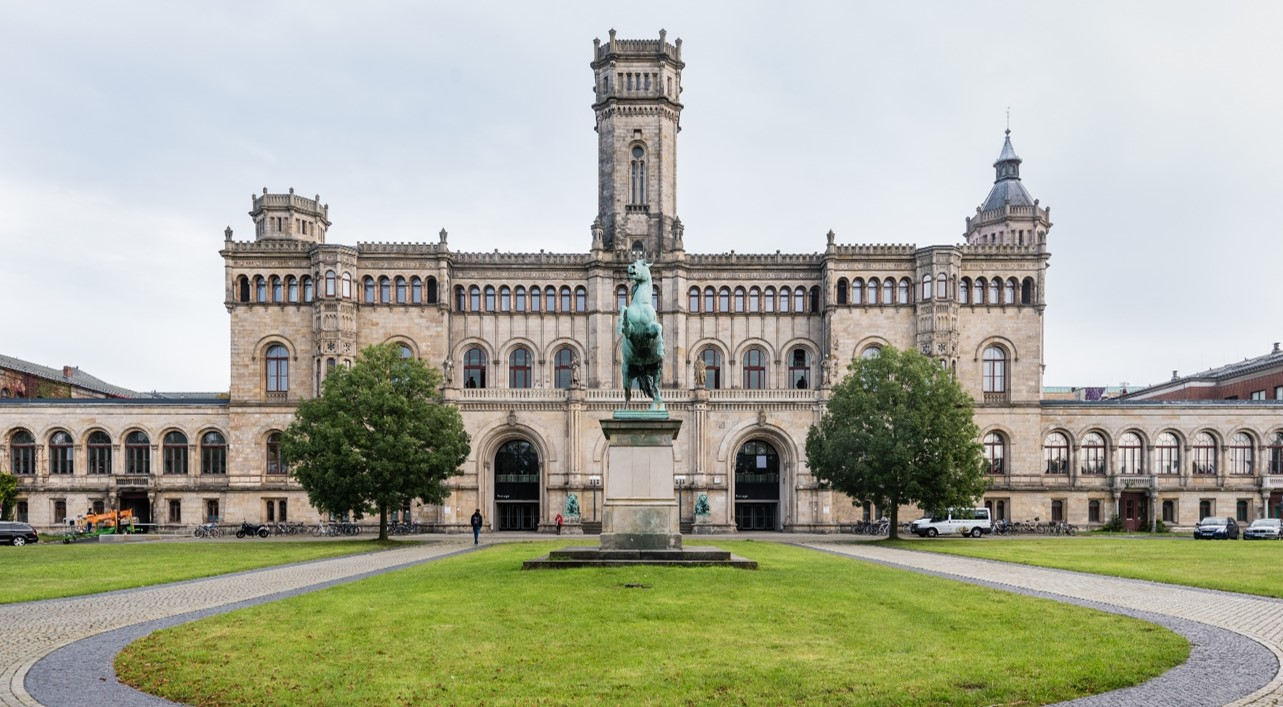
\includegraphics[width=0.65\textwidth]{figures/luh_default_presentation_title_image.jpg}}

% Title page: luhstyle
% \setbeamertemplate{title page}[luhstyle]
% % Add optional title image here
% \addtitlepageimage{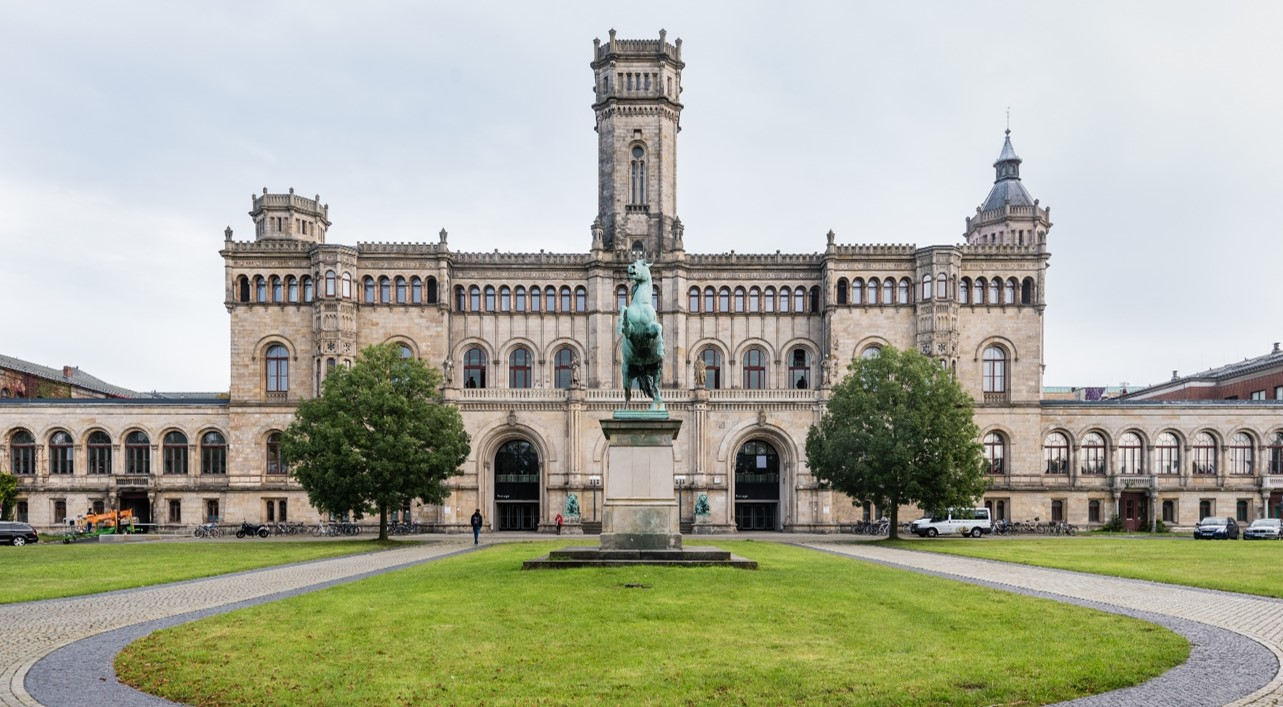
\includegraphics[width=0.75\textwidth]{figures/luh_default_presentation_title_image.jpg}}

\author[Lindauer \& Anand]{Marius Lindauer and Avishek Anand\\[1em]
	
\includegraphics[height=\logoheight]{../latex_main/figures/luh_logo_rgb_0_80_155.pdf}\qquad

\includegraphics[height=\logoheight]{../latex_main/figures/TNT_darkv4}\qquad

\includegraphics[height=\logoheight]{../latex_main/figures/L3S.jpg}	}
\date{Winter Term 2021
}


%%% Custom Packages
%----------------------------------------------------------------------
% Create dummy content
\usepackage{blindtext}

% Adds a frame with the current page layout. Just call \layout inside of a frame.
\usepackage{layout}


\title[Introduction]{iML: Interpretable Models}
\subtitle{Methods}

%\institute{}


\begin{document}
	
	\maketitle

	%-----------------------------------------------------------------------------------------------------------------------------

\begin{frame}[c]{Linear Regression}

    $$y = w_0 + w_1 x_1 + w_2 x_2 + \ldots + w_p x_p + \epsilon $$

    \begin{itemize}
        \item $y$ output
        \item $w_i$ weight of input feature $x_i$
        \item $\epsilon$ remaining error (e.g., because of noise)
        \item[$\leadsto$] model consists of $p+1$ weights $w_i$
        \item Properties and assumptions:
        \begin{itemize}
            \item linear
            \item normality assumption of the target
            \item homoscedastic (i.e., constant variance)
            \item independence of features
            \item fixed features (i.e., free of noise)
            \item no strong correlation of features
        \end{itemize} 
    \end{itemize}

\end{frame}

%------------------------------------------------------------------
%------------------------------------------------------------------

\begin{frame}[c]{Interpretation of Linear Regression}

    $$y = w_0 + w_1 x_1 + w_2 x_2 + \ldots + w_p x_p + \epsilon $$

    Let's consider different feature types:
    \begin{itemize}
        \item Numerical features: Increase of numerical value will lead to $w_i$ times increased output
        \item Binary feature: Either weight $w_i$ is active (1) or not (0).
        \item Categorical feature: One-hot-encoding of $L-1$ new features for $L$ categories
        \item Intercept $w_0$: reflects expected features values if features were standardised (0-mean, 1-stdev)
    \end{itemize}	
    \pause
    Feature importance:
    \begin{itemize}
        \item t-statistic by the estimated weight scaled with its standard error\\ (i.e., less certain about the correct value)
    \end{itemize}
    $$t_{w_i} = \frac{w_i}{SE(w_i)} $$
\end{frame}

%------------------------------------------------------------------
%------------------------------------------------------------------
	
\begin{frame}{Logistic Regression}

    $$P(y = 1) =\frac{1}{1 + \exp(-( w_0 + w_1 x_1 + w_2 x_2 + \ldots + w_p x_p ))} $$

    \begin{itemize}
        \item Probabilistic \alert{classification} model 
        \item Typically, we set the threshold to $0.5$ to predict 
        \begin{itemize}
            \item Class 1 if $P(y=1) > 0.5$
            \item Class 0 if $P(y=1) \leq 0.5$
        \end{itemize}
    \end{itemize}	

\end{frame}

%------------------------------------------------------------------
%------------------------------------------------------------------

\begin{frame}[c]{Interpretation of Logistic Regression}

    $$\log \left(\frac{P(y = 1)}{P(y=0)}\right) = w_0 + w_1 x_1 + w_2 x_2 + \ldots + w_p x_p  $$

    \begin{itemize}
        \item weights relate to log odds-ratio
        \item Again linear in log odds-ratio
        \item[$\leadsto$] change by one unit changes the odds ratio by a \alert{factor} of $\exp(w_i)$.
        \medskip
        \pause
        \item Interpretation for different feature types is the same as for linear regression
    \end{itemize}	

\end{frame}

%------------------------------------------------------------------
%------------------------------------------------------------------

\begin{frame}{GLM and Interactions}

    \begin{itemize}
        \item Linear models are often too restrictive for many applications
    \end{itemize}
    
    \medskip
    Non-Gaussian outputs via Generalized Linear Models (GLMs):
    $$g(\mathrm{E}_Y (y\mid x)) = w_0 + w_1 x_1 + w_2 x_2 + \ldots + w_p x_p$$
    \begin{itemize}
        \item link function $g$ -- can be freely chosen
        \item exponential family defining $\mathrm{E}_Y$ -- can be freely chosen
        \item weighted sum $X^\top W$
    \end{itemize}
    
    \medskip 
    \pause
    Interaction effects via feature engineering:
    \begin{itemize}
        \item E.g., feature expansion: $w_{x_i,x_j} x_i \cdot x_j$
    \end{itemize}
    
\end{frame}

%------------------------------------------------------------------
%------------------------------------------------------------------

\begin{frame}{Generalized Additive Models (GAMs)}

Non-Linear relations can be addressed by:
    \begin{itemize}
        \item feature transformations (e.g., exp or log)
        \item Categorization of features (i.e., intervals / buckets of feature values)
        \item GAMs:
    \end{itemize}
    
    $$g(\mathrm{E}_Y (y\mid x)) = w_0 + f_1(x_1) + f_2(x_2) + \ldots + f_p(x_p)$$
    
    \begin{itemize}
        \item instead of $w_i x_i$ use flexible functions $f_i(x_i)$ $\leadsto$ splines
    \end{itemize}

\end{frame}

%------------------------------------------------------------------
%------------------------------------------------------------------

\begin{frame}{Decision Trees}

\begin{columns}

\begin{column}{0.3\textwidth}

   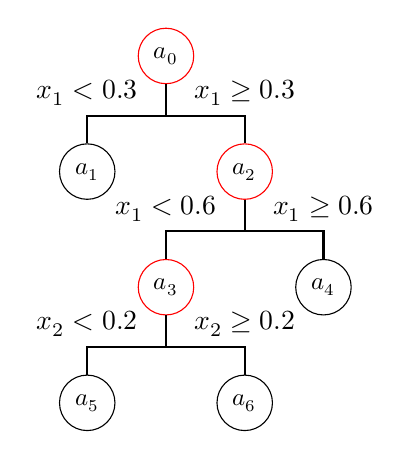
\begin{tikzpicture}
   \usetikzlibrary{arrows}
    \usetikzlibrary{shapes}
     \tikzset{treenode/.style={draw, circle, font=\small}}
     \tikzset{line/.style={draw, thick}}
     \node [treenode, draw=red] (a0) {$a_0$};
     \node [treenode, below=0.75cm of a0, xshift=-1cm]  (a1) {$a_1$};
     \node [treenode, draw=red, below=0.75cm of a0, xshift=1cm]  (a2) {$a_2$};
     
     \node [treenode, draw=red, below=0.75cm of a2, xshift=-1cm] (a3) {$a_3$};
     \node [treenode, below=0.75cm of a2, xshift=1cm]  (a4) {$a_4$};
     
     \node [treenode, below=0.75cm of a3, xshift=-1cm] (a5) {$a_5$};
     \node [treenode, below=0.75cm of a3, xshift=1cm]  (a6) {$a_6$};
     
     \path [line] (a0.south) -- + (0,-0.4cm) -| (a1.north) node [midway, above] {$x_1<0.3$};
     \path [line] (a0.south) -- +(0,-0.4cm) -|  (a2.north) node [midway, above] {$x_1\geq0.3$};
     
     \path [line] (a2.south) -- + (0,-0.4cm) -| (a3.north) node [midway, above] {$x_1<0.6$};;
     \path [line] (a2.south) -- +(0,-0.4cm) -|  (a4.north) node [midway, above] {$x_1\geq0.6$};
     
          
     \path [line] (a3.south) -- + (0,-0.4cm) -| (a5.north) node [midway, above] {$x_2<0.2$};;
     \path [line] (a3.south) -- +(0,-0.4cm) -|  (a6.north) node [midway, above] {$x_2\geq0.2$};
     
   \end{tikzpicture}

\end{column}

\begin{column}{0.7\textwidth}

Properties:
\begin{itemize}
    \item able to model non-linear effects
    \item terminal nodes (aka leaf nodes) can have several observations and predicts the mean outcome over these
    \item Applicable to regression and classification
\end{itemize}

Interpretation:
\begin{itemize}
    \item directly by following the tree (i.e., sequence of rules)
    \item Feature importance by (scaled) score of much the splitting criterion was reduced compared to the parent
\end{itemize}

\end{column}

\end{columns}

\end{frame}

%------------------------------------------------------------------
%------------------------------------------------------------------

\begin{frame}[c]{Decision Rules}

\texttt{IF COND$_1$ AND COND$_2$ AND ... THEN value}

\begin{itemize}
    \item \texttt{COND$_i$} can be of the form \texttt{feature <op> value} where \texttt{<op>} can be for example $\{=, <, > \}$
\end{itemize}

\pause
\medskip

Properties:
\begin{description}
    \item{Support} Fraction of observations to support appliance of rule
    \item{Accuracy} for predicting the correct class under the condition(s)
\end{description}

$\leadsto$ often trade-off between these two

\pause
\medskip

$\leadsto$ many different ways to learn a set of rules (incl. a default rule if none of the rules are met)

\end{frame}

%------------------------------------------------------------------
%------------------------------------------------------------------

\begin{frame}[c]{Other Interpretable Models}

\textbf{RuleFit} \lit{Friedman and Popescu 2008}{https://arxiv.org/abs/0811.1679}
\begin{itemize}
    \item Combination of linear models and decision trees 
    \item Allows for feature interactions and non-linearities
\end{itemize}

\textbf{NaiveBayes}
$$P (C_k \mid x ) = \frac{1}{Z} P(C_k) \prod_{i=1}^{n} P(x_i \mid C_k) $$
\begin{itemize}
    \item product of probabilities for a class on the value of each feature
    \item strong independence assumption
\end{itemize}


\textbf{k-Nearest Neighbor}
\begin{itemize}
    \item (closely related to case-based reasoning)
    \item Average of of the outcome of neighbors -- local explanation
\end{itemize}

\end{frame}
	
\end{document}
